\subsection*{Άσκηση 6}

Έστω απλό $k$-συνεκτικό γράφημα $G$ με $n$ κορυφές και ελάχιστο βαθμό κορυφής $\delta(G)$.

\begin{enumerate}[(i)]
\item Δείξτε ότι αν $\delta(G) \ge n-2$ τότε $k = \delta(G)$.
\item Βρείτε απλό γράφημα $G$ με $\delta(G) = n - 3 $ και $k < \delta(G)$.
\end{enumerate}

\subsubsection*{Λύση}

\begin{enumerate}[(i)]
\item 

Aν $\delta(G) = n-1$ τότε προφανώς ισχύει αφού αν αφαιρέσουμε $n-2$ κορυφές απο πλήρη γράφο, οι υπόλοιπες
θα συνδέονται. Αν $\delta(G) = n-2$ τότε κάθε κορυφή δεν θα συνδέεται το πολύ με μία άλλη. Αν αφαιρέσουμε
$n-3$ κορυφές αυτές που απομένουν θα πρέπει να συνδέονται διαφορετικά μία απο αυτές δε θα συνδέονταν 
με 2 κορυφές.

\item
    Για $n=5$ υπάρχει το αντιπαράδειγμα του παρακάτω γράφου.

        \begin{center}
        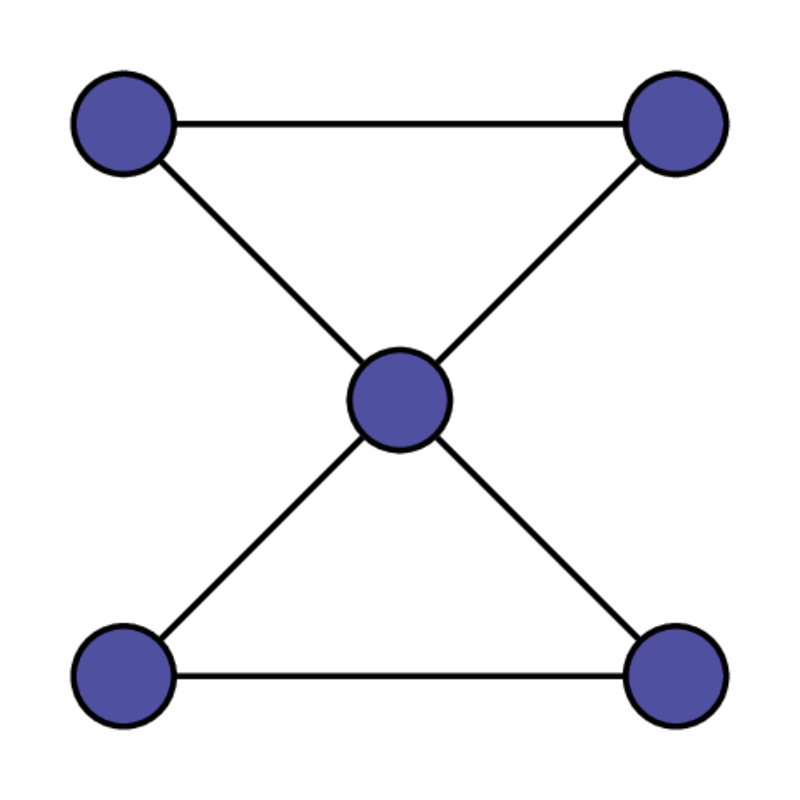
\includegraphics[height=6cm, width=.3\textwidth]{exercise6/diagrams/d1.png}
        \end{center}

\end{enumerate}
